\documentclass[lang=cn]{elegantpaper}


\usepackage{array}
\usepackage{courier}
\usepackage{xcolor}
\usepackage{tabulary}
\usepackage{float}
\usepackage{makecell}
\usepackage{multirow}
\usepackage{zhnumber}
% \usepackage{cite}

\title{智能手机传感器的国内外发展情况及其应用}
\author{郁文啸,高博飞,韩奕南}
\institute{(北京邮电大学计算机学院)}

\version{}
\date{\zhtoday}

\newcommand{\ccr}[1]{\makecell{{\color{#1}\rule{1cm}{1cm}}}}

\begin{document}

\maketitle

% 摘要
\begin{abstract}
传感器(transduce/sensor)在现代工业、农业、生产生活中的应用无处不在。随着信息技术的发展,特别是5G通信的普及,智能化的脚步大大加快,无人驾驶,人工智能、万物互联开始由设想逐步走向现实,智能手机在智能化的过程中起到了重要的作用。作为实现自动化、智能化的基础和首要环节,传感器的应用将更加广泛。人们希望手机能够变成功能强大的便携式电子设备,传感器在智能手机中也得到了越来越普遍的应用。本文以智能手机上的传感器为重点研究对象,侧重分析了国内外智能手机传感器的发展情况以及应用。
    \keywords{传感器;智能手机;发展;应用}
\end{abstract}

\section{引言}

智能手机技术的发展速度快得令人难以想象,传感器技术在手机中的应用让我们的生活方式发生重大转变。十多年前,手机中的传感器用量开始增长。除了麦克风,首先是图像传感器进入手机,随后是惯性传感器、光学传感器、压力传感器和气体传感器等,集成的传感器越来越多。与传统手机相比,智能手机的优势非常明显,不仅有高分辨率的摄像头、灵敏方便的触摸屏,也有安全有效的指纹识别、高效精准的GPS,更有便捷的蓝牙和NPC等。传感器在手机中的广泛使用给智能手机带来了翻天覆地的变化,手机里各式传感器的发展一日千里,在未来,传感器的种类必将更为繁多,功能也会更为复杂,精确度也会大幅度提升。


\section{通讯类传感器}

\subsection{蓝牙}

蓝牙是一种无线通讯技术标准,用来让固定与移动设备,在短距离间交换资料,以形成个人局域网(PAN)。

1999年出现了第一代蓝牙技术。蓝牙规范1.0版本主要是针对点对点的无线数据传输,给出了标准的数据传输分组格式以及分组类型。随后的1.1版本将1.0版本的点对点扩展为点对多点的数据传输,并修正了前一版本中错误和模糊的概念。蓝牙技术1.2版本的传输速率与1.1版本相同,但实现了设备识别的高速化,增强了数据传输的抗干扰能力,与现有的1.1版本完全兼容,确保其向后兼容1.1版本的产品。蓝牙协议规范1.2版本中有以下的改进和增强:更加快速地连接、自适应跳频、扩展的同步面向连接链路、增强的错误检测与信息流、增强的同步能力、增强的流规范等,这些改进可以增加数据传输的抗干扰性和可靠性,为其实时传输提供了有力支撑。

2004年出现了第二代蓝牙技术。蓝牙2.0版本增加了增强型数据速率(EDR)协议,大大提高了蓝牙技术数据传输的性能,数据传输速率可达1.2版本传输速率的3倍。蓝牙2.1+EDR标准在2.0版本的基础上对数据传输的性能加以改善,具有3个主要特征:改善装置配对流程、节约能源和增强安全性等。

2009年出现了第三代蓝牙技术。蓝牙3.0+HS采用交替射频技术,并且集成了IEEE 802.11协议适应层,使蓝牙数据传输速率提高至24Mbit/s。此外,还增加了单播无连接数据传输模式和增强功率控制等新功能。

2010年出现了第四代蓝牙技术。蓝牙4.0规范,提出了“低功耗蓝牙”、“传统蓝牙”和“高速蓝牙”三种模式。

2013年,蓝牙技术联盟推出蓝牙4.1规范,支持多设备连接和智能连接。

2014年,蓝牙技术联盟推出了蓝牙4.2规范。\cite{BlueTooth}

2016年出现了第五代蓝牙技术。蓝牙5.0在有效传输距离上是4.2LE版本的4倍,传输速度将是4.2LE版本的2倍。蓝牙5.0还支持室内定位导航功能,针对物联网进行了很多底层优化。2019年,蓝牙技术联盟推出了蓝牙5.1规范。

2020年,蓝牙技术联盟推出了蓝牙5.2规范。

\subsection{NFC}

NFC指近距离无线通信,又简称近距离通信或近场通信,是一套通信协议,让两个电子设备在相距几厘米之内进行通信。NFC是飞利浦公司发起,由诺基亚、索尼等厂商联合主推的一项无线技术。

2002年,NFC被批准成为ISO/IEC IS 18092国际标准,此后还被批准为EMCA-340标准与ETSI TS 102 190标准。NFC标准与ISO/IEC 14443和ISO/IEC 15693非接触式IC卡兼容。

Philips在非接触IC卡方面是业界领头者,其Mifare芯片卡技术广泛使用于世界几个大型交通运输系统上,也使用在VISA信用卡等金融服务上。而Sony的Feli Ca芯片卡技术在中国香港及深圳、新加坡、日本的市场占有率非常高,主要应用于交通及金融机构。两种技术的融合,将可以扩大非接触IC卡的应用范围。

为了推动NFC的发展和普及,飞利浦、索尼和诺基亚创建了一个非赢利性行业协会NFC论坛,旨在促进NFC技术的实施和标准化,确保设备和服务之间协同合作。目前,论坛在全球拥有80多个成员,包括万事达国际、VISA、微软、摩托罗拉、NEC、松下电工、三星、德州仪器和VISA国际。\cite{BlueTooth2}

2006年6月, 诺基亚和中国移动、飞利浦、易通卡公司在厦门启动中国首个NFC手机支付试验。用户使用内嵌NFC模块的诺基亚3220手机, 可在任何一个易通卡覆盖的营业网点(公交、汽车、轮渡、电影院、快餐店)进行手机支付\cite{NFC}。

2010年11月,AT\&T、T-Mobile 和 Verizon 联手成立了一个智能手机无线支付联盟 Isis。

\subsection{GPS位置传感器}

全球定位系统是美国国防部研制,美国太空军运营与维护的中距离圆型轨道卫星导航系统。

全球定位系统由美国政府于1970年代开始进行研制,1978年2月首次发射,并于1994年全面建成。使用者只需拥有GPS接收芯片即可使用该服务。GPS信号分为民用的标准定位服务和军用的精确定位服务两类。

中国为北斗卫星导航系统制定了“三步走”发展规划,从1994年开始发展的试验系统为第一步,2004年开始发展的正式系统为第二步。至2012年完成对亚太大部分地区的覆盖并正式提供卫星导航服务,此战略的前两步已经完成。根据计划,北斗卫星导航系统第三步将在2018年覆盖“一带一路”国家,2020年完成,届时将实现全球的卫星导航功能。


\section{物理信息类传感器}

物理信息类传感器指能够侦测环境中物理信息的传感器,包括图像传感器、声音传感器、触摸传感器、加速度传感器、陀螺仪、光线传感器、距离传感器、霍尔传感器、磁场传感器、温度传感器、气压传感器等。

\subsection{图像传感器}

图像传感器,或称感光元件,能将光学图像转换成电子信号。智能手机中的图像传感器即指摄像头。

\subsubsection{图像传感器的发展历史}

1873年,科学家约瑟·美及伟洛比·史密夫就发现了硒元素结晶体感光后能产生电流;20世纪50年代,光学倍增管出现;1965年至1970年,IBM、Fairchild等企业开发出光电二极管和双极二极管阵列;1970年,贝尔实验室发明CCD图像传感器,依靠其高量子效率、高灵敏度、低暗电流、高一致性、低噪音等性能,成为图像传感器市场的主导;90年代末,CCD时代逐渐落幕,图像传感器步入CMOS时代。

现代CMOS图像传感器性能已经十分优越。2017年索尼XZ1系列使用的IMX400可达1900万像素;2018年华为P20 Pro使用的IMX600可达4000万像素;2021年华为P50更是达到了惊人的5000万像素。

\subsubsection{国内外图像传感器比较}

索尼、三星、豪威是CMOS的三巨头,仅在2016年,这三个厂商的市场占有率之和就达到了72\%。在行业应用上,索尼有STARVIS和Pregius两个主打技术。在产品上,索尼已经建立了业界最完善的CMOS产品线,涵盖各个领域,把持住中高端领域的市场份额。

国内的CMOS传感器厂商在规模和技术上与国外厂商还存在一定的差距,产品主要用于中低端消费类电子领域。但是,一些国内领先的CMOS传感器厂商如思比科、格科微等,依托其自主核心技术,正逐步扩大份额、向中高端市场渗透。

\subsection{声音传感器}

声音传感器是与人类耳朵相似的具有频率反应的电子元件,能将机械能波转换成电能波。智能手机中的声音传感器即指麦克风。

\subsubsection{麦克风的发展历史}

1857年,斯科特发明了语言描记器,利用振动的针尖在纸板上记录下音波;1876年埃尔米贝林纳·发明了碳精电极麦克风;1886年,爱迪生发明了第一个实用的碳粒式麦克风;1916年,贝尔实验室的文特发明了电容式麦克风;1931年,贝尔实验室的文特和图拉斯发明了动圈式麦克风;1966年,舒尔公司推出了SM58,其至今仍被认为是现场演唱麦克风的行业标准;随着电子技术的发展,麦克风向数字化、高频化、多功能化和轻薄便携化的方向发展。

现代麦克风主要分为动圈式和电容式两种。动圈麦被广泛应用于KTV或演出等娱乐场合,成本低、使用简单,但声音不够细腻,细节不够丰富。电容麦被广泛应用于专业的人声演唱,灵敏度高、频响宽、瞬时响应快、声音还原度高。智能手机中的麦克风通常是MEMS麦克风,体积小,声音的指向性强。

\subsubsection{国内外麦克风比较}


MEMS麦克风产业链主要包括“设计、制造、封装、测试”4个重要环节,设计和制造难度较大,往往体现MEMS厂商的核心竞争力,而封装和测试难度较小,易于掌握。所以很多中国厂商首先从封装和测试做起,逐步掌握核心芯片技术。

2010年,美国楼氏电子在全球MEMS麦克风市场中处于绝对领先地位,市场份额超过80\%。中国厂商以购买英飞凌裸芯片进行封装和测试的方式进入MEMS麦克风领域。 随着近些年中国MEMS麦克风厂商的长足进步,2019年,楼氏电子的市场份额下滑至36\%,以歌尔股份、瑞声科技、敏芯股份、共达电声股份有限公司为代表的中国厂商也成为全球MEMS麦克风的主要参与者。由于中美贸易战愈演愈烈,海外供应体系受到种种限制,以智能手机为代表的智能终端厂商更加重视国内产业链的建设,因此,中国MEMS麦克风厂商的发展速度继续提升,有望进一步扩大市场份额。

\subsection{触摸传感器}

触摸传感器是基于电容感应的触摸开关模块,当人体或金属直接触碰到传感器上的金属面时,就可以被感应到。智能手机中的触摸传感器即指触摸屏。

\subsubsection{触摸屏的发展历史}

1965年,E.A.johnson发明第一个手指式触摸屏;1970年,G.Samuel Hurst发明第一个电阻触摸屏;1982年,多伦多大学研制出首例人控多点触控装置;1984年,贝尔实验室研究出多点触控屏;1993年,IBM和BellSouth推出第一台触屏电话;2002年,索尼引入了相互的电容接触识别;2007年,苹果推出了iPhone,从此,触屏手机逐渐成为时代主流。

现代触摸屏主要有四种,分别为电阻式、表面声波式、红外线式以及电容式\cite{touchScreenClassify},每一种触摸屏都有其各自的优缺点。电阻式触摸屏透光率较高,但寿命不长久;表面声波式触摸屏有极好的防刮性,最适合公共场合使用;红外线式触摸屏价格低廉、安装方便,但分辨率较低;电容式触摸屏耐磨性好、耗电量低,现代智能手机通常也采用电容式触摸屏。

\subsubsection{国内外触摸屏比较}

目前市面上手机使用TFT-LCD或OLED屏幕,其中OLED已经逐步发展为主流,而OLED多采用电容屏技术。韩国的三星和LGD占据了OLED产能的大半江山,顶尖技术还是掌握在韩国厂商手中,而且在主流量产的6世代面板中,韩国厂商产能表现也非常突出。大陆厂商最近几年不断追逐,在产能方面已经成长为第二大集团。中国大陆厂商在6代面板中表现也有一定突破,日本和中国台湾的厂商的产能与技术能力则逐步落后。


\subsection{运动传感器}

智能手机中的运动传感器包括三轴加速度传感器和三轴角速度传感器(陀螺仪)。三轴加速度传感器可以侦测智能手机在三个不同方向上的加速度,陀螺仪可以侦测到智能手机的旋转。三轴陀螺仪和三轴加速度传感器可以组合构成六轴的运动传感器,它基本上可以检测到所有形式的运动,包括速度、方向、位移等参数。

\subsubsection{运动传感器的发展历史}

1852年,法国物理学家傅科研制出世界上第一台傅科陀螺仪;1908年,德国科学家赫尔曼·安许茨·肯普费设计了一种单转子摆式陀螺罗经;20世纪50年代,美国麻省理工的查尔斯·施塔克·德雷珀研制出单自由度液浮陀螺仪;20世纪60年代初,美国人罗伯特·克雷格研制出了动力调谐陀螺仪;1964年,美国研制出静电陀螺仪;1963年,美国斯佩里公司研制出激光陀螺仪;进入20世纪90年代,随着微机电和量子技术的不断发展,核磁共振陀螺仪和原子干涉陀螺仪等新型陀螺仪得到了快速发展。

现代智能手机中的加速度计主要采用MEMS惯性传感器,MEMS惯性传感器在1990年代开始规模应用在汽车工业和国防工业,20世纪初开始应用于手机等消费电子领域。

\subsubsection{国内外运动传感器比较}

MEMS制造目前主要分为三类,纯MEMS代工、IDM企业代工和传统集成电路MEMS代工。国内MEMS代工厂华润上华、中芯国际、上海先进等,硬件条件虽与国际水平相近,但开发能力远不及海外代工厂。目前Honeywell在MEMS陀螺研制开发领域是世界上最高水平之一。经过多年的发展,国内MEMS传感器设计行业已积累一批人才,但与国际领先的企业相比,国内MEMS传感器设计行业高端、专业人才仍相对稀缺。

\subsubsection{运动传感器的应用}

运动传感器可以跟踪并捕捉3D空间的完整动作,常见应用包括实现计步、“摇一摇”功能、体感技术以及VR视角的调整与侦测等。不仅如此,它还可以用于识别交通流拥挤程度:从智能手机运动传感器中的加速度计和三轴陀螺仪模块提取加速度和角加速度参数,与手机的GPS数据相结合,共同作为交通流状态估计参数,可以提高交通流拥挤状态判别的精度和可靠性。\cite{DetectTrafiic}

\subsection{重力传感器}

智能手机中的重力传感器和通常利用压电效应实现,能够感知重力、静态姿势(躺着、俯、立着、左侧、右侧,可以精确测量倾角)。三轴重力感应在静止状态下会测到1G的重力加速度,把这个加速度分配到3个轴[x,y,z]上得到不同数值大小,计算可得三轴与水平的相对角度。\cite{GSensorTraditionnalUsage}

随着移动网络的不断提速,重力传感器的作用也不再仅仅局限于实现手机横屏竖屏转换,国内外有许多学者也在研究重力传感器的新型应用。如重力传感器可以用于实现用户身份认证,通过收集用户的行为数据,计算分析用户的行为特征,用于识别用户身份是否合法,减轻用户的记忆负担。\cite{GSensorUsage}

\subsection{其它物理信息类传感器}

\subsubsection{光线传感器}

光线传感器,也就是感光器,能够感知周围光的明暗程度,将光信号转成电信号。有了光线传感器,智能手机可以根据所处环境的光线来调节手机屏幕的亮度,既保护眼睛又达到省电的目的。\cite{TraditionalUsageOfSendor}

中国光线传感器市场存在低端产品产能过剩、低端产品同质化现象严重、传感器制造企业国际竞争力低的问题。中国光线传感器行业上游及中游企业缺乏对核心、高端技术的掌握,导致行业发展与国际发展水平存在差距。

\subsubsection{距离传感器}

距离传感器由一个红外LED灯和红外辐射光线探测器构成。大多数智能手机中的距离传感器和光线传感器是放在一起的,位于手机听筒周围。用户在通电话时手机会靠近耳朵,系统根据距离传感器的信息会自动关闭显示屏,防止误触。手机在兜里时,距离感应器还可以防止手机被无意唤醒,若是忘记息屏,系统也会自动触发保护机制。

\subsubsection{磁场传感器}

磁场传感器是利用磁阻来测量平面磁场,从而检测出磁场强度以及方向位置。一般应用于指南针或是地图导航中,帮助手机用户实现准确定位。

磁场传感器排名前15位的制造商占有85\%的市场份额,日本、德国、荷兰、瑞士、比利时是该市场的主要成员。

\subsubsection{霍尔传感器}

霍尔传感器安装在手机上主要功能就是使用智能皮套(磁皮套),扣上皮套后屏幕就会在皮套上留出的小窗口中出现一个小窗口界面,用来接听来电或阅读短信。

目前全球霍尔传感器的主要生产集中在欧美日地区,主要消费地区为中国,美国,欧洲,日本等地区。

\subsubsection{温度传感器}

许多智能手机都配置有温度传感器,如果发现某一部件温度过高,手机就会关机,防止手机损坏。

智能手机里的温度传感器不仅可以用于测量内部器件的温度,只要采用了合适的算法,它甚至能测量环境温度。有研究学者指出,采用补偿表法进行环境温度测量,在部分产品上的测试精度能达到$\pm$1℃\cite{Temperature}。

\subsubsection{气压传感器}

气压传感器原理是将薄膜与变组器或电容连接在一起,当气压产生变化时,电阻或电容数值也发生变化,从而将气压信息转化为电信号。气压传感器可以用于测量海拔高度,计算用户爬了几楼等。实验表明,智能手机中的气压传感器在实现楼层定位时,定位精度能达到85\%\cite{storeyDetect}。


\section{生物信息类传感器}

生物信息类的传感器包括心率传感器、血氧传感器、指纹传感器。

\subsection{指纹传感器}

\subsubsection{指纹传感器的发展}

对于传统的指纹按键手机,目前主流的技术是电容式指纹传感器,然而超声波指纹传感器也有逐渐流行起来趋势。电容式指纹传感器作用时,手指是电容的一极、另一极则是硅芯片数组,透过人体带有的微电场与电容传感器之间产生的微电流,指纹的波峰波谷与传感器之间的距离形成电容高低差,来描绘出指纹的图形。而超音波指纹传感器原理也类似,但不会受到汗水、油污的干扰,辨识速度也更为快速。运用在手机中可用来解锁、加密、支付等等。

伴随手机全面屏概念的流行,市场主流手机开始采用屏下指纹识别技术。屏下指纹识别技术是通过屏幕玻璃下方完成指纹识别解锁过程的新技术。屏下指纹识别主要利用超声波、光学等技术穿透各种不同的材质,从而达到识别指纹的目的。\cite{UsageWid}

\begin{figure}[H]
    \centering
    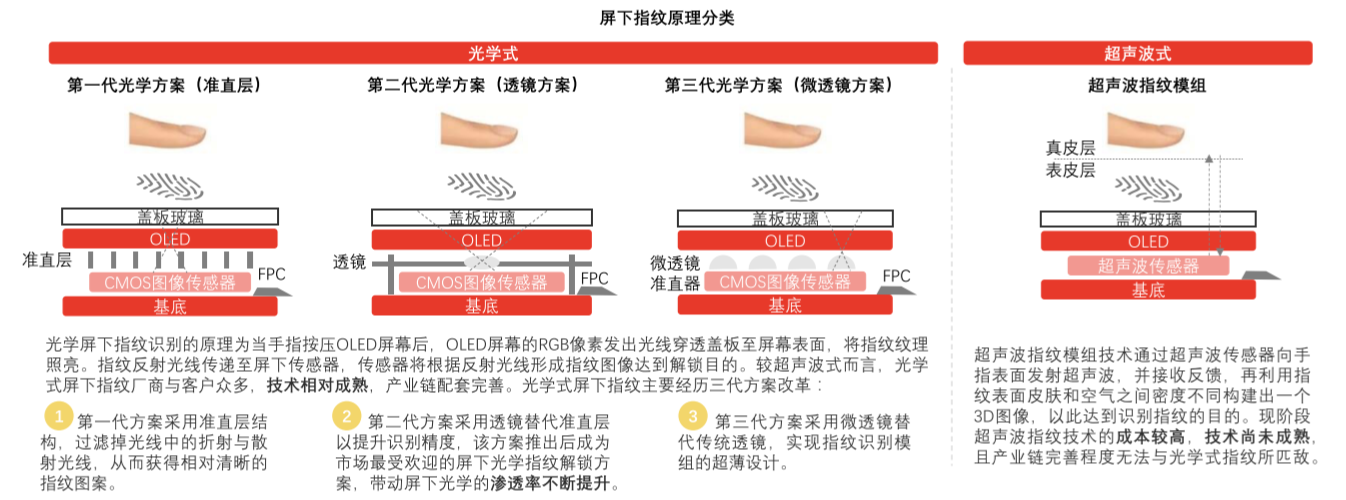
\includegraphics[width=1.0\textwidth]{1-1.png}
    \caption{屏下指纹原理分类}
    % \label{fig:屏下指纹原理分类}
\end{figure}

\subsubsection{指纹传感器的未来需求}

5G智能手机催生超薄屏下指纹解锁方案需求。现阶段,光学式屏下指纹的指纹模组厚度较大,因此模组在安装时需与电池交错分布,才可将足够光路空间预留给透镜。 因此,该指纹方案的安装位置大多接近设备下方,且会压缩电池空间。5G时代下,智能手机搭载的5G芯片功率较大,射频前端等器件用量与电池容量的提升导致手机 内部空间将更加紧凑,对于智能手机设备的零件空间要求较为苛刻。超薄光学式屏下指纹技术可有效满足模组搭载的厚度要求。由于该方案的模组厚度极薄,因此可叠放与电池与屏幕之间,为5G设备提供更大电池容量空间。

\subsection{心率传感器}

\subsubsection{国内外心率传感器比较}

国内一般采用光学心率传感器。血液中血细胞的浓度会随着心脏的跳动而变化,光学心率传感器的主要原理是将光线 照射到人类的皮肤中,观测血液颜色的变化,从而利用光电传感器将这种变化转为电信号, 一般将此种技术命名为光电容积脉搏波描记法测心率技术,简称PPG。

国外的如苹果手机,主要采用PPG以及电极传感测量方式。电极式提取的是完整的心电图,而不是一个简单的心率信息,心电图中有很多详细的健康信息,例如P Q R S T五个波形,是医生用来判断心脏健康的依据。\cite{Heart}电极式的目前有三个电极和二个电极方案,也即需要三个触点和两个触点(需要三手指或双手指触控)来读取数据,所以,这样就不能主动读取数据,这是电极式的最大问题,因为需要消费者有意识地去测量,而不能自动不间断测量并上传数字,更不能实现远程监控。

\subsubsection{心率传感器的跳转}

光电式心率传感器挑战很大,受环境影响很大,甚至不同的肤色都会影响信号链路,更不用说运动。所以,光电式需要在后端电路做大量的处理,包括运动去除功能等。

\subsection{血压、血氧传感器}

通常情况下,手机上的血氧传感器有两个不同光波长的LED,一个是红色,另一个则是红外线。而其原理是含氧量正常的血液和缺氧的血液对光的吸收不同,含氧的血液会吸收更多的红外线,缺氧的血液则会让更多的红外线通过。这使得血氧仪能够快速、无创的检测氧气水平\cite{BloodO2},并测量氧气被传输到四肢的情况。

目前主流的技术是基于光电容积脉搏波描记法测心率技术(PPG)。




% 自动生成引用
% \bibliographystyle{unsrt}
\bibliography{Ref}

\end{document}